\centering
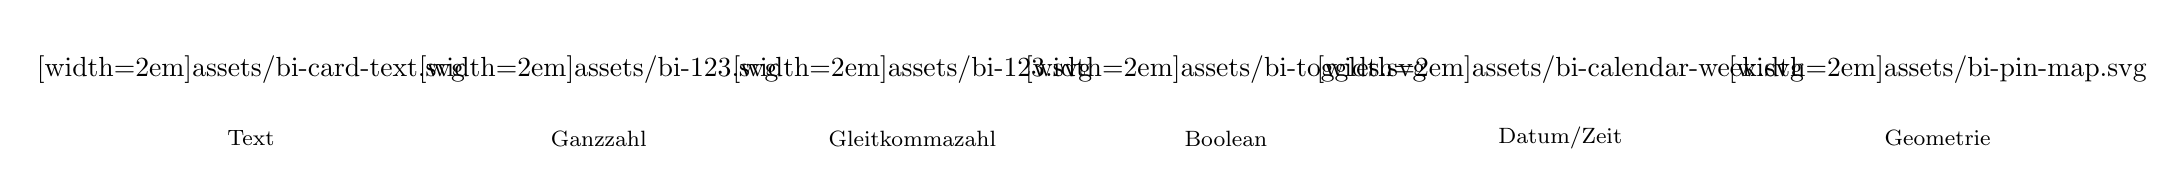
\begin{tikzpicture}
  \tikzset{icon/.style={outer xsep=4.5em, outer ysep=1em, minimum height=3em}}
  \tikzset{label/.style={font=\footnotesize}}
  \node [icon] (text)  at (0, 0)       {\includesvg[width=2em]{assets/bi-card-text.svg}};
  \node [icon] (int)   at (text.east)  {\includesvg[width=2em]{assets/bi-123.svg}};
  \node [icon] (float) at (int.east)   {\includesvg[width=2em]{assets/bi-123.svg}};
  \node [icon] (bool)  at (float.east) {\includesvg[width=2em]{assets/bi-toggles.svg}};
  \node [icon] (dt)    at (bool.east)  {\includesvg[width=2em]{assets/bi-calendar-week.svg}};
  \node [icon] (geom)  at (dt.east)    {\includesvg[width=2em]{assets/bi-pin-map.svg}};
  \node [label] at (text.south)  {Text};
  \node [label] at (int.south)   {Ganzzahl};
  \node [label] at (float.south) {Gleitkommazahl};
  \node [label] at (bool.south)  {Boolean};
  \node [label] at (dt.south)    {Datum/Zeit};
  \node [label] at (geom.south)  {Geometrie};
\end{tikzpicture}
